\chapter{Plochy a ich vlastnosti}

\label{kap:plochy} % id kapitoly pre prikaz ref

V tejto kapitole opíšeme spôsoby zadania funkcií, ich vlastnosti, 
ako aj základné definície a vety, ktoré budeme v práci používať \cite{filo_rostas}.

\section{Funkcia daná implicitne}

\begin{definition}
    Nech $A \subseteq \mathbb{R}^n$, $B \subseteq \mathbb{R}$ sú neprázdne množiny. 
Hovoríme, že na množine $A$ je definovaná funkcia viacerých premenných
$f$, ak je daný predpis, ktorý každej n-tici $(x_1, . . . , x_n)$
z množiny $A$ priradí práve jeden prvok $f(x_1, . . . , x_n)$ z množiny $B$.
Zapisujeme 
$$f : A \to B,$$
$$(x_1, . . . , x_n) \mapsto f(x_1, . . . , x_n).$$
Ak premennú $y \in B$ vyjadríme ako funkčnú hodnotu bodov $(x_1, . . . , x_n) \in A$
$$f : y = f(x_1, . . . , x_n),$$
hovoríme o explicitnom zadaní funkcie.
\end{definition}


Pri explicitne zadanej funkcii je závislá premenná $y \in \mathbb{R}$ vyjadrená ako funkčná hodnota nezávislých
premenných $(x_1, . . . , x_n)\in\mathbb{R}^n$.
\\*
Funkcia zadaná implicitne je daná pomocou funkcie $$F : \mathbb{R}^n \times \mathbb{R} \to \mathbb{R},$$
$$(x_1, . . . ,x_n, y) \mapsto F(x_1, . . . , x_n, y),$$ ktorá každému prvku $(x_1, . . . ,x_n, y) \in \mathbb{R}^{n} \times \mathbb{R}$ 
priradí určitú hodnotu \mbox{$F(x_1, . . . , x_n, y) \in \mathbb{R}$.}
Implicitne definovaná funkcia je daná nulovou hladinou tejto funkcie, teda bodmi $(x_1, . . . , x_n, y)$, 
ktoré vyhovujú rovnici $$F(x_1, . . . , x_n, y) = 0.$$  
Táto rovnica určuje vzťah medzi závislou premennou $y \in \mathbb{R}$
a nezávislými premennými $(x_1, . . . , x_n) \in \mathbb{R}^n$. 

\begin{note}
    Ak $f : \mathbb{R}^n \to \mathbb{R}$, $f: y = f(x_1, . . . , x_n)$ je funkcia a body
    $(x_1, . . . , x_n, y) \in \mathbb{R}^n \times \mathbb{R}$ vyhovujúce implicitnej rovnici
        \begin{equation}
        \label{eq:graph_of_implicit_function}
        y - f(x_1, ..., x_n) = F(x_1, . . . , x_n, y) = 0
        \end{equation}
    sú grafom funkcie f,
    potom je funkcia f implicitne zadaná rovnicou \ref{eq:graph_of_implicit_function}.
\end{note}

Teda pre každú explicitne zadanú funkciu existuje implicitná rovnica, ktorá ju určuje.
Naopak to však neplatí. Nie každá implicitná rovnica určuje vzťah pre jedinú explicitne zadanú
funkciu. Príkladom je implicitná rovnica pre jednotkovú kružnicu $x^2 + y^2 - 1 = 0$. 

V našej práci sa zaoberáme algoritmami triangulácie grafov implicitne definovaných funkcii v 
$\mathbb{R}^3$. Odteraz
budeme pracovať iba s funkciami pre $n = 2$. Grafy takýchto funkcii sú špeciálne \textit{plochy}. 
Ďalej bude platiť, že $x$ a $y$ sú nezávislé premenné a $z$ je závislá premenná.

Aj keď sa implicitné funkcie nedajú vždy vyjadriť explicitne, pre každú spojite diferencovateľnú
implicitnú funkciu platí, že na nejakom okolí takmer každého bodu, existuje explicitná funkcia,
ktorou sa dá vyjadriť.
O tom nám hovorí nasledujúca veta.

\begin{theorem}
 (o funkcií danej implicitne pre $\mathbb{R}^3$)
 
 Nech funkcia $F: \mathbb{R}^3 \to \mathbb{R}$ je spojite diferencovateľná. 
 Nech $(x_0, y_0, z_0) \in \mathbb{R}^3$ je bod taký, že $F(x_0, y_0, z_0) = c$.
 Ak $$\frac{\partial F}{\partial z} (x_0, y_0, z_0) \neq 0$$ potom existuje okolie 
 bodu $(x_0, y_0, z_0)$ také, že ak $(x, y)$ je dostatočne blízko $(x_0, y_0)$, 
 tak v tomto okolí existuje jediná funkcia $z = z(x ,y)$ spĺňajúca implicitnú rovnicu
 $F(x, y, z(x, y)) = c$. Navyše platí $z(x_0, y_0) = z_0$.
\end{theorem}

Pomocou explicitne zadanej funkcie nevieme vyjadriť veľa reálnych objektov, 
vieme vyjadriť len ich časti, ktoré treba následne zlepiť, 
preto je funkcia daná implicitne pri vykresľovaní plochy veľmi obľúbená. 
Implicitne definované plochy majú oproti explicitným veľkú výhodu napríklad
v CSG modelovaní. Vďaka CSG modelovaniu vieme vytvárať pomerne komplexné
modely len používaním booleovských operácií (zjednotenie, prienik, rozdiel)
a geometrických transformácií. Tieto operácie sa aplikujú veľmi jednoducho, ak
máme plochy zadané implicitne.


\begin{note}
    Z vety o funkcií danej implicitne navyše vyplýva, že ak je $z = z(x,y)$ definovaná na nejakom 
    zúžení definičného oboru funkcie F podľa predchádzajúcej vety, tak $z$ je spojitá funkcia v 
    premennej x aj v premennej y. 
\end{note}

\newpage

\section{Vlastnosti funkcie danej implicitne}
\label{kap:implicit_surface_properties}

Vlastnosti plôch sú dôležité pri každom algoritme modelujúcom tieto plochy. Využívame ich napríklad na detekciu ostrých hrán, 
zisťovanie zakrivenia funkcie, ale aj pri rôznych dodatočných úpravách výsledkov základných algoritmov.
Ak nepoznáme vyjadrenie funkcie $z(x, y)$, môžeme jej vlastnosti získať z jej implicitnej rovnice $F(x, y, z) = 0$.


\begin{theorem}
    (derivácia funkcie danej implicitne)

    Parciálne derivácie funkcie $z(x, y)$ danej implicitne rovnicou F(x, y, z) = 0 možno vypočítať pomocou vzorca
    $$\frac{\partial z(x, y)}{\partial x} = -\frac{\frac{\partial F}{\partial x}}{\frac{\partial F}{\partial z}}$$
    a podobne 
    $$\frac{\partial z(x, y)}{\partial y} = -\frac{\frac{\partial F}{\partial y}}{\frac{\partial F}{\partial z}}.$$
\end{theorem}

Normála k ploche definovanej implicitne funkciou $F(x,y,z)$ v bode $(x_0, y_0, z_0)$ je definovaná ako (jednotkový) 
gradient implicitnej funkcie  v tomto bode.

\begin{definition}
    Nech $f : \mathbb{R}^3 \to \mathbb{R}$ je spojite diferencovateľná funkcia. Gradient tejto 
    funkcie je definovaný ako 
    $$\nabla F(x, y, z) = (\frac{\partial F(x, y, z)}{\partial x}, \frac{\partial F(x, y, z)}{\partial y}, 
    \frac{\partial F(x, y, z)}{\partial z})$$
    a normálový vektor ako normovaný gradient
    $$N(F(x, y, z))  = \frac{\nabla F(x, y, z)}{\| \nabla F(x, y, z) \|} \,\,\,\,\,\, pre \,\,\,\,\,\,
    \nabla F(x,y,z) \neq 0.$$
    \\*
    Gradient tejto funkcie v bode $(x_0, y_0, z_0)$ vypočítame dosadením 
    $$\nabla F(x, y, z)\big|_{(x_0, y_0, z_0)}$$ 
    a normálový vektor podobne ako $$N(F(x, y, z))\big|_{(x_0, y_0, z_0)}.$$
\end{definition}

Tento výpočet gradientu, resp. normálového vektora môžeme použiť iba ak poznáme parciálne derivácie funkcie $F$ v danom bode.
V opačnom prípade musíme použiť numerické metódy na výpočet gradientu. Najčastejšie metódy používané na tento problém sú 
\textit{symetrická} alebo \textit{asymetrická diferencia}. V tejto práci ďalej predpokladáme, že poznáme parciálne derivácie funkcie $F$.

Pre regulárnu, implicitne definovanú plochu navyše môžeme konzistentne definovať \textit{vnútro}
ako množinu $\{x \in \mathbb{R}^3 | F(x)<0 \}$ a \textit{vonkajšok} ako množinu 
$\{x \in \mathbb{R}^3 | F(x)>0 \}$.

O tomto fakte pre konečnú, uzavretú, regulárnu plochu hovorí 
\textit{Jordanova-Brouwerova veta o separácii}~\cite{montiel2009curves}. Navyše podľa tejto 
vety platí, že \textit{vnútro} je konečná množina a \textit{vonkajšok} je nekonečná množina. 
Pre nekonečnú, regulárnu, implicitne definovanú plochu sú obe množiny nekonečné. 


\section{Singulárne body a krivky}

Singulárne body implicitne definovanej plochy sú také body, kde $\nabla F(x, y, z) = 0$. Tieto body nemusia byť nutne izolované, 
v takom prípade hovoríme o singulárnych krivkách. 

Singulárne body a krivky sa vyskytujú napríklad pri CSG modelovaní. 

Jednoduchý príklad izolovaného singulárneho bodu a 
singulárnej krivky môžeme vidieť na obrázku~\ref{obr:singular_points}. Singulárne
body kužeľa sú na obrázku vyznačené červenou. Vrchol kužeľa je izolovaným singulárnym bodom, keďže v 
každom jeho dostatočne malom okolí sú všetky ostatné body regulárne. Príkladom neizolovaných singulárnych
bodov, teda singulárnej krivky sú body na spoji podstavy s plášťom kužeľa. Tieto singulárne body tvoria 
singulárnu krivku -- kružnicu.

\begin{figure}
    \centerline{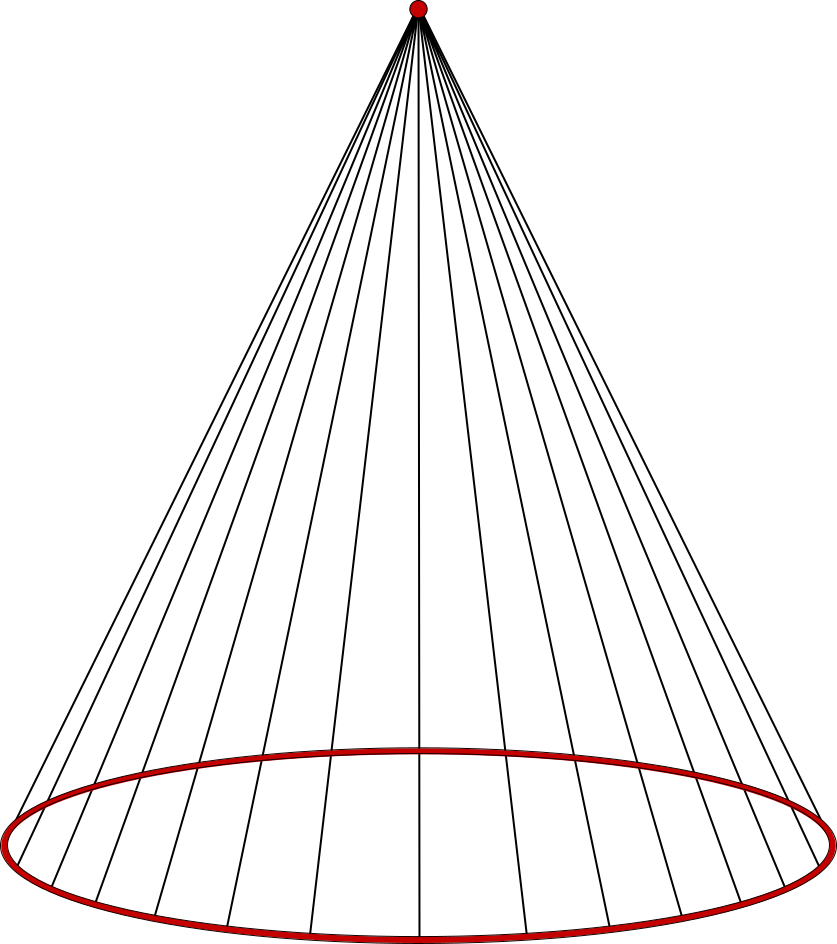
\includegraphics[width=0.3\textwidth]{images/singular_points}}
    \caption[Singulárny bod a singulárna krivka]
    {Singulárny bod a singulárna krivka ilustrovaná na kuželi.}
    %id obrazku, pomocou ktoreho sa budeme na obrazok odvolavat
    \label{obr:singular_points}
\end{figure}

Pri CSG modelovaní vznikajú singulárne body a krivky na priesečníkoch plôch. Príklad
singulárnej krivky vyskytujúcej sa pri CSG modelovaní môžeme vidieť na obrázku~\ref{obr:singular_curves}, 
táto krivka je priesečník guľových plôch, takisto kružnica.

\begin{figure}
    \centerline{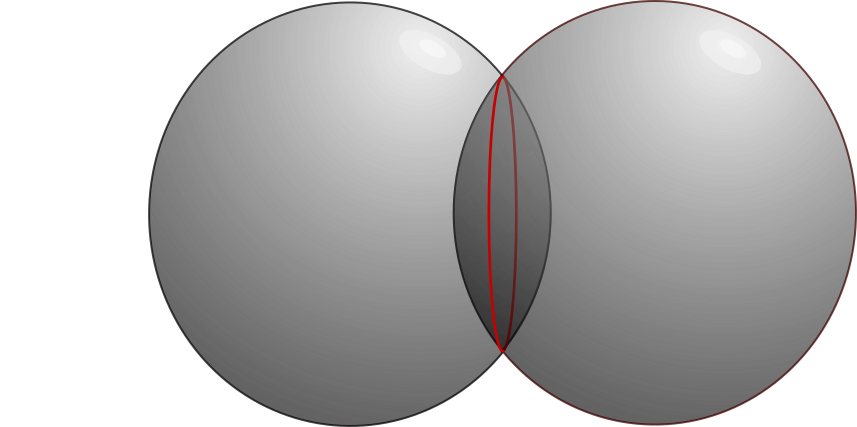
\includegraphics[width=0.45\textwidth]{images/singular_curves}}
    \caption[Singulárna krivka na priesečníku dvoijce sfér]
    {Singulárna krivka na priesečníku dvoijce sfér.}
    %id obrazku, pomocou ktoreho sa budeme na obrazok odvolavat
    \label{obr:singular_curves}
\end{figure}